\subsection{\idx{IMS} Demonstrator} % (fold)
\label{sub:demonstrator}

\begin{figure}[htbp]
  \centering
  \subfigure[System architecture]{
    \label{fig:ims-arch}
    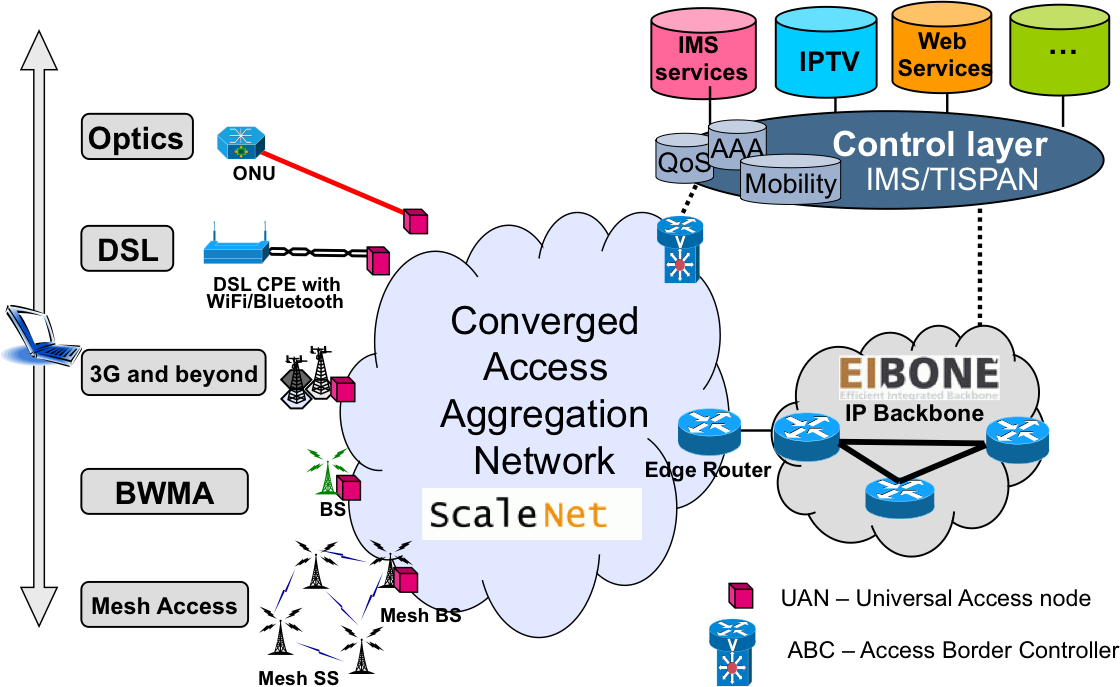
\includegraphics[width=\textwidth]{ims-arch}
  }
  \subfigure[Architecture of the demonstrator]{
    \label{fig:ims-arch-real}
    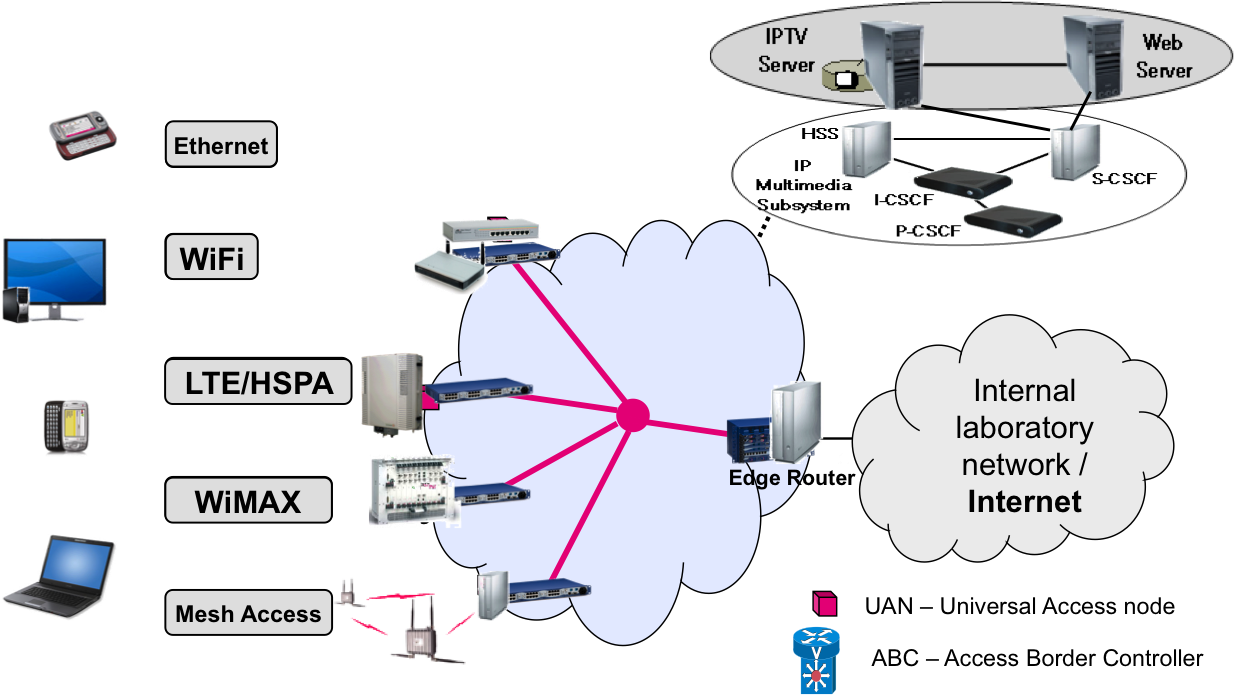
\includegraphics[width=\textwidth]{ims-arch-real}
  }
  \caption{IMS architecture}
  \label{fig:ims}
\end{figure}

In the offices of \ida{T-Labs} in Berlin and Darmstadt there is a demonstrator with a working implementation of \idx{ScaleNet}.
That demonstrator is composed by several servers and a network infrastructure that enables access to the system using different network protocols and devices.
In Figure~\vref{fig:ims-arch-real} the actual network and hardware are exposed, replacing the same space as in the logical view (Figure~\vref{fig:ims-arch}).

\begin{figure}[htbp]
  \centering
    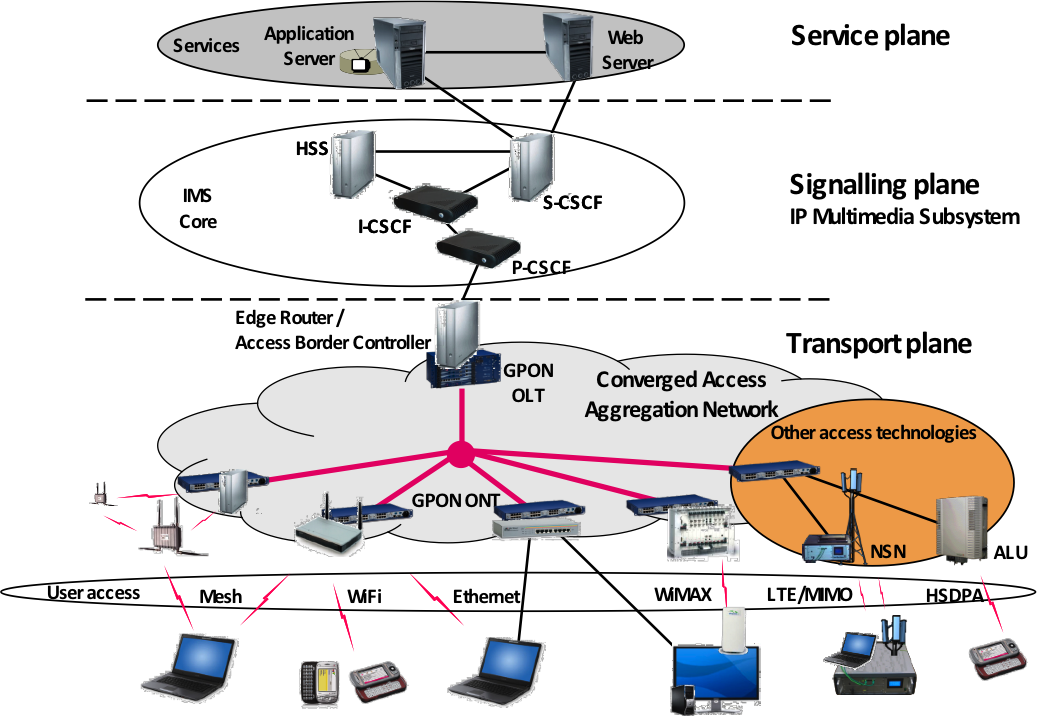
\includegraphics[width=\textwidth]{ims-setup}
  \caption{Setup of the demonstrator}
  \label{fig:ims-setup}
\end{figure}

Figure~\vref{fig:ims-setup} describes the setup in a better way and highlights the three different planes of the demonstrator.
The developed web application is executed from the \idx{Web Server} and the \idx{Application Server}, since it belongs to the service plane.
The signaling plane has also to be taken into account, because it communicates directly with the servers.

However, that is not the real deployment of the hardware used.
Whether for convenience or efficiency, tasks are distributed between two main servers.
This does not affect the logic of the system, since those tasks could be easily decoupled in an alternate deployment with more servers.
Anyway, the interesting pieces of hardware for this project are:

\begin{description}
  \item[\ida{IMS} core] This machine contains the \ida{IMS} server\footnote{The IMS core is open source software from Fraunhofer FOKUS and it can be freely downloaded from: \url{http://www.openimscore.org/}}, but since the \ida{IMS} load is not very high, it is responsible for other things.
  It acts as a \idx{Web Server} (using \idx{Apache} Web Server\footnote{\url{http://httpd.apache.org/}}) serving \ida{PHP} applications.
  It is also the internal \ida{DNS} server.
  \item[\idx{Application Server}] This is the \ida{IPTV} server, where the video content is streamed.
  It is also a \idx{Web Server}, but it serves \idx{Java} applications based on the \ida{OSGi} framework\footnote{\url{http://www.osgi.org/}}.
  \item[User Devices] Devices intended for the user to access the services.
  There is a TV, a laptop and several phones.
  All of them run a custom \ida{IMS} client that holds a connection to the servers, allowing the identification and adding \ida{IPTV} and \ida{VoIP} capabilities to those devices.
  In the last phase of the development, an \idx{iPhone} was added for testing purposes.
\end{description}

This demonstrator contains several demo applications running.
The interesting one for this project is the application that handles \ida{IPTV} streaming.

% subsubsection demonstrator (end)